\section{Gap decomposition and CertiFlip}\label{sec:gap}


\begin{theorem}\label{thm:gap}
Let $y\ge0$, $r=c-A^\top y$, and let $\mathcal C$ be a clustering that separates all
far pairs.  Then
\begin{equation}\label{eq:gap}
\cost(\mathcal C)-\LB(y)=\sum_{e\in P}\underbrace{\big(r_ex^{\mathcal C}_e-\min\{0,r_e\}\big)}_{g_e\ge0}
+\sum_i\underbrace{y_i\,(a_i^\top x^{\mathcal C}-b_i)}_{s_i\ge0}.
\end{equation}
\end{theorem}
\begin{proof}
$\cost(\mathcal C)=K+c^\top x^{\mathcal C}=K+r^\top x^{\mathcal C}+y^\top
Ax^{\mathcal C}$.  Subtract~\eqref{eq:lb}.  Each $g_e\ge0$ because
$x_e\in\{0,1\}$, and each $s_i\ge0$ by the validity of row $i$.
\end{proof}

A pair term vanishes iff the clustering agrees with the sign of the reduced
cost.  A row term vanishes iff the row is tight or has multiplier $0$.
Assigning each term to the endpoints of its pairs gives a \emph{gap map} over
the vertices.

\begin{corollary}[local certificate]\label{cor:local}
For $B\subseteq V$ let $\Gamma_B(\mathcal C)$ be the sum of the terms
of~\eqref{eq:gap} whose pair, or one of whose row pairs, has an endpoint in
$B$.  Let $\mathcal C'$ be any clustering that separates far pairs and
coincides with $\mathcal C$ on all pairs with both endpoints outside $B$.  Then
$\cost(\mathcal C)-\cost(\mathcal C')\le\Gamma_B(\mathcal C)$.  In particular,
if $\Gamma_B(\mathcal C)<1$ then no re-clustering of $B$ improves $\mathcal C$.
\end{corollary}
\begin{proof}
Apply~\eqref{eq:gap} to both clusterings.  Terms not touching $B$ coincide,
and the terms of $\mathcal C'$ are non-negative.  Costs are integers.
\end{proof}

\paragraph{Gap-guided LNS.}  Large-neighbourhood search~\citep{Shaw98}, here
with exact sub-MIPs in the spirit of RINS and local
branching~\citep{DannaRL05rins,FischettiL03local}, fixes
the clustering outside a vertex set $B$ ($|B|\le 60$) and re-optimises $B$
exactly.  Let $\mathcal K$ be the outside clusters with a positive edge into
$B$.  Re-clusterings of $B$ correspond to clusterings of $B$ together with one
super node per $K\in\mathcal K$, where super nodes must stay apart.  The cost is
$\sum_{uv}[uv\in\Ep]x_{uv}+[uv\notin\Ep](1-x_{uv})$ for $u,v\in B$, plus
$w_{vK}x_{vK}+(|K|-w_{vK})(1-x_{vK})$ for each $v\in B$, where $w_{vK}$ counts
the positive edges between $v$ and $K$.  We solve this MIP with HiGHS and add
triangle inequalities lazily until the solution is transitive.  To keep
Corollary~\ref{cor:local} applicable, $v$ may join $K$ only if it is within
distance two of every member of $K$, and far pairs inside $B$ are fixed apart.
Neighbourhoods are grown around high-gap vertices, either by breadth-first
search or as a union of whole clusters.  Neighbourhoods with $\Gamma_B<1$ are
skipped because they are certified optimal.  Theorem~\ref{thm:gap} and
Corollary~\ref{cor:local} need a clustering that separates far pairs, which
the output of the flipping search need not do.  Before the search, and after
every improvement, we therefore move to a singleton every vertex $v$ with
$|N(v)\cap S|<(|S|-1)/2$ in its cluster $S$, until there is none.  Each such
move lowers the cost, and by the argument of Lemma~\ref{lem:half} the result
separates all far pairs.  The certificate $\Gamma_B<1$ covers re-clusterings
of $B$ that also separate far pairs; by Lemma~\ref{lem:half} these include
every optimal one.

Figure~\ref{fig:gapmap} shows the gap map at work on the neighbourhood of
Figure~\ref{fig:support}.  For a Pivot clustering the gap of 10 is
concentrated on one cluster; the LNS re-optimises the blocks around the
high-gap vertices and reaches a clustering whose cost equals the bound, which
certifies it optimal.

\begin{figure}[!tbp]
\centering
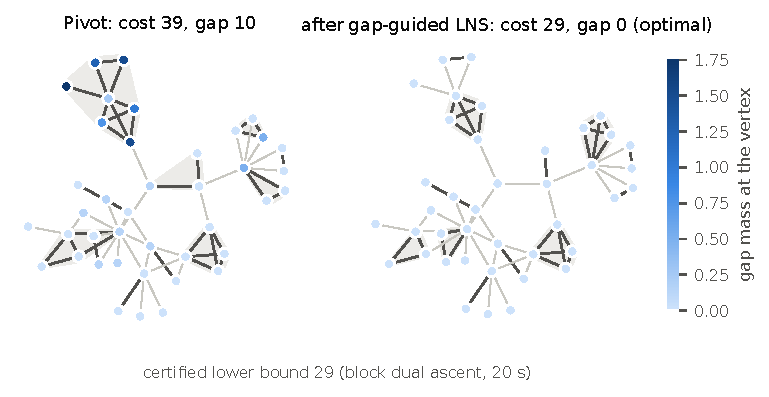
\includegraphics[width=0.92\textwidth]{figures/fig_gapmap.pdf}
\caption{Gap decomposition (Theorem~\ref{thm:gap}) on the neighbourhood of
Figure~\ref{fig:support}.  Each vertex is coloured by its share of
$\cost(\mathcal C)-\LB$ (pair terms split between the endpoints, row terms
between the vertices of the row); shaded regions are clusters, dark edges lie
inside a cluster.  Left: a Pivot clustering.  Right: after gap-guided LNS the
gap is zero, so the clustering is optimal.  Computed by the released code.}
\label{fig:gapmap}
\end{figure}


\subsection{CertiFlip}\label{sec:algo}

\begin{algorithm}[t]
\caption{CertiFlip$(G^+,T)$}\label{alg:certiflip}
\begin{algorithmic}[1]
\State $\mathcal C\gets\textsc{Pivot}(G^+)$ with a uniformly random order
\State $\mathcal C\gets\textsc{IteratedFlip}(\mathcal C)$ \Comment{insertion local search with flips}
\State build the distance-two support $P$
\State $y\gets$ star packing with ruin-and-recreate local search \Comment{feasible dual}
\State $y\gets\textsc{BlockAscent}(P,y,\mathcal C)$ \Comment{METIS sweeps, then gap-guided blocks}
\If{one block covered $V$ and separation converged}
  \State $\mathcal C\gets$ best of $\mathcal C$ and \textsc{IteratedFlip}(\textsc{CMSY-Round}$(x^\star)$) over several roundings
\EndIf
\State $\mathcal C\gets\textsc{GapLNS}(\mathcal C,y)$ until time $T$
\State \Return $\mathcal C$ and $\lceil\LB(y)\rceil$ \Comment{lines 4--5 share half of the budget $T$}
\end{algorithmic}
\end{algorithm}

\paragraph{Insertion local search.}  For every root $r$ we build one candidate
insertion $S(r)$ by \emph{cleaning} $N[r]$.  Starting from $S=N[r]$, we
repeat a few sweeps over $v\in N[r]\setminus\{r\}$: we put $v$ in $S$ iff
joining $S$ costs $v$ less than staying in the remainder of its current
cluster.  Both costs are computed exactly from counts of weighted positive
neighbours.  We then compute the exact change of the objective in
$O(\sum_{v\in S}\deg v)$ time and apply the insertion if it is negative.
Rounds of insertions alternate with a multilevel (Louvain-type) vertex-move
local search.  That search works on the weighted objective, moves super nodes
at coarse levels and hence also merges clusters.  \textsc{IteratedFlip}
follows \citet{CohenAddadLPTYZ24}.  Positive weights take values in
$\{1,1.5,2\}$ (we double all weights to stay in integers).  Each round flips
the pairs cut by the previous solution, re-optimises, flips and re-optimises
again, and combines the last three solutions with their $3$-way pivot.  The
best candidate under the original objective is returned.

\begin{theorem}\label{thm:certiflip}
Let $\mathcal C$ and $\LB$ be the output of Algorithm~\ref{alg:certiflip}.
\begin{enumerate}
\item[(a)] $\mathbb E[\cost(\mathcal C)]\le3\,\OPT$.
\item[(b)] $\LB\le\OPT$, so $\cost(\mathcal C)/\lceil\LB\rceil$ is an upper
bound on the approximation ratio achieved on the instance.
\item[(c)] If line~7 is executed, $\mathbb E[\cost(\mathcal C)]\le 2.06\,\OPT$.
\end{enumerate}
\end{theorem}
\begin{proof}
Every step after line~1 returns a clustering no worse than its input: the
local searches only apply improving moves, \textsc{IteratedFlip} returns the
best of its candidates, which include the local optimum reached from its input,
and \textsc{GapLNS} accepts only improvements.  (a) then follows from the
Pivot guarantee~\citep{AilonCN08}.  (b) is Theorem~\ref{thm:anytime}(a) and
the integrality of $\OPT$.  (c) If one block covered $V$ and separation
converged, the block LP primal $x^\star$ satisfies all
rows~\eqref{eq:t1}--\eqref{eq:t2}, so it is feasible for $\mathrm{LP}_P$.  Its
cost is the value of the block LP.  Every row of the block LP is valid for an
optimal clustering (Lemma~\ref{lem:half} and Proposition~\ref{prop:subgraph}),
whose cut vector is therefore feasible for the block LP; hence the block LP
value is at most $\OPT$.  By Theorem~\ref{thm:sparse}(b,c),
$\mathbb E[\cost(\textsc{CMSY-Round}(x^\star))]\le 2.06\,\OPT$.  The remaining
steps are monotone.
\end{proof}

\begin{remark}
Part~(a) holds for any procedure that starts from a Pivot clustering and never
makes its solution worse; it is a safeguard, not a distinguishing property.
If the insertion local search reached an optimum with respect to
\emph{all} cluster insertions, \citet{CohenAddadLPTYZ24} would give a factor of
$2$, and $2-2/13$ with enough flipping rounds.  Our candidate generation
explores a polynomial subfamily of insertions, so we do not claim these
factors.  The certificate of Theorem~\ref{thm:certiflip}(b), however, is
valid in every case.
\end{remark}

\paragraph{Running time.}  Pivot takes $O(n+m)$ time.  One round of insertions
takes $O(\sum_v\sum_{u\in N(v)}\deg u)=O(\sum_u\deg(u)^2)$, the same order as
the size of $P$ and the number of bad triangles.  The support takes
$O(\sum_w\deg(w)^2)$ time and memory.  The block LPs dominate the running
time, and the time spent on them is set by the budget $T$.


\paragraph{Budget.}  The budget $T$ is checked between steps: before each
block LP, each LNS neighbourhood and each flipping round.  A single round of
the insertion local search, the construction of the support and a sub-MIP
are not interrupted, so a run can exceed $T$.  Section~\ref{sec:exp} reports
the measured wall-clock and CPU times of every run, including these overruns,
and the time at which the final bound was reached.
